\documentclass[12pt,a4paper]{article}

\usepackage{graphicx}
\usepackage{booktabs}
\usepackage{amsmath}
\usepackage{url}
\usepackage{xcolor}

\graphicspath{{figures/}{../resultsAct4/}}

\begin{document}

\title{\textcolor{black}{\LARGE\bfseries Distributed Matrix Multiplication
using MPI\\[0.5em]
\normalsize\normalfont Individual Assignment 4 --- Report}}
\author{\textcolor{black}{Carlos Montesdeoca Vega\\[8pt]
\texttt{repository:}\\[2pt]
\small\texttt{https://github.com/CarlosMontesdeoca21/BasicMatrixMultiplication}}}
\date{\textcolor{black}{November 16, 2026}}

\maketitle

\begin{abstract}
This report investigates how the number of worker processes affects the
performance of a dense matrix multiplication distributed with MPI, and how the
distributed version compares with its sequential baseline and with the
shared-memory OpenMP implementation. We distribute the classic i-j-k triple
loop (double precision) with a 1-D row-block partitioning of the result
matrix: \texttt{MPI\_Scatterv} distributes contiguous row blocks of A,
\texttt{MPI\_Bcast} sends the full B to every worker, and
\texttt{MPI\_Gatherv} collects the rows of C, with each phase timed
separately. Inputs are deterministic shared matrices up to $n = 1500$; worker
counts $p \in \{1, 2, 4, 8, 16, 22\}$ are measured 5 times after 2 warm-ups,
reporting medians and interquartile ranges. Strong scaling saturates at
$p = 8$: the best end-to-end speedups are $4.93\times$ ($n = 1000$) and
$5.77\times$ ($n = 1500$) over the sequential baseline, with efficiency
falling from $0.62$--$0.72$ at $p = 8$ to $0.21$--$0.20$ at $p = 22$. The
transfer phase grows from $0.05\%$ of end-to-end time at $p = 1$ to $21\%$ at
$p = 22$ ($n = 1500$), dominated by broadcasting the full B matrix, while the
compute-only speedup peaks at $6.82\times$. On this single physical machine
the OpenMP reference reaches $8.49\times$ ($n = 1000$, 16 threads), yet for
$n = 1500$ the packed MPI buffers outperform OpenMP by up to $1.30\times$.
All 260 measurements validate with exactly zero elementwise difference
against the sequential reference. Conclusions are limited to the tested
hardware, inputs and configurations; local multi-worker execution was
authorized by the professor.
\end{abstract}

\section{Introduction}
\label{sec:intro}

Matrix multiplication is a fundamental operation in scientific computing and
data analytics. Its classical algorithm has cubic time complexity
($O(n^3)$) and poor cache behavior, making it computationally expensive.
Distributing the work across processes is the standard way to scale it
beyond a single memory domain. The goal of this work is to evaluate the
performance of a distributed implementation built with MPI, and to answer
focused research questions: how does the worker count affect the end-to-end
execution time compared with the sequential baseline, where does the strong
scaling saturate, how is the time split between transfer, computation and
gathering, and how does the distributed version compare with the
shared-memory OpenMP version measured in the same campaign?

The hypotheses registered before the measurements were:
\begin{itemize}
\item \textbf{H1:} Strong scaling will be sub-linear and will saturate well
below $p = 22$, because the local computation per worker shrinks as $1/p$
while the communication (in particular the broadcast of the full B matrix to
every worker) grows with $p$.
\item \textbf{H2:} Communication will be a small fraction of the end-to-end
time for large problems at low worker counts, but will become visible
(above 10\%) at high worker counts; the smallest problem
($n = 100$) will be overhead-dominated, so adding workers beyond a small
count will \emph{increase} the end-to-end time.
\item \textbf{H3:} On a single physical machine the distributed version will
generally trail the OpenMP version at high worker counts (per-process data
copies and collective calls versus a shared address space), although the
contiguous packed buffers required by MPI may let it win for the largest
tested size.
\end{itemize}

We implement and compare three approaches:
\begin{itemize}
\item Sequential algorithm (classic i-j-k triple loop in C, double
precision, row-pointer storage) --- the baseline validated in Activity 1;
\item Parallel execution using OpenMP (the same i-j-k kernel, parallelized
over the rows of the result matrix) --- the Activity 3 implementation,
re-measured inside this campaign for a fair comparison;
\item Distributed execution using MPI (the same arithmetic on contiguous
row blocks distributed over $p$ processes, with the three phases timed
separately).
\end{itemize}

All experiments use the same input matrices per configuration, a documented
measurement protocol with warm-up runs and repetitions, and robust
statistics (median and interquartile range).

\section{Code and organization}
\label{sec:code}

The project repository includes a structured hierarchy with implementations
under the \texttt{Activity4/code} folder alongside management scripts:
\begin{itemize}
\item \textbf{C benchmark (\texttt{benchmark\_mpi.c}):} Contains the three
kernels (\texttt{Sequential} i-j-k, \texttt{OpenMP} with
\texttt{\#pragma omp parallel for} over rows, and the \texttt{MPI} kernel),
plus a CSV loader, checksum validation and a memory metric based on the
process API (\texttt{psapi}). The MPI path implements a 1-D row-block
partitioning: rank 0 loads A and B, \texttt{MPI\_Scatterv} distributes
contiguous row blocks of A, \texttt{MPI\_Bcast} sends the full B to every
rank, each rank multiplies its block into a contiguous C buffer, and
\texttt{MPI\_Gatherv} returns the rows of C. Transfer, compute and gather are
timed separately with \texttt{QueryPerformanceCounter}; end-to-end time is
their sum, with a barrier before each repetition. Per-process memory is
gathered with \texttt{MPI\_Gather} so the reported value is the maximum over
all workers.
\item \textbf{Python automation scripts:} \texttt{generate\_inputsAct4.py}
creates the deterministic input matrices (uniform values in $[0,1)$, seed
42, sizes $n \in \{10, 100, 500, 1000, 1500\}$), \texttt{run\_sweep\_act4.py}
orchestrates the whole campaign through \texttt{mpiexec} (self-test,
validation, then every size/method/worker combination),
\texttt{validate\_act4.py} checks the sequential result against NumPy,
\texttt{merge\_results\_act4.py} computes medians, IQR, strong scaling,
phase medians and efficiency, and \texttt{plot\_results\_act4.py} exports the
performance charts.
\item \textbf{Data artifacts:} Raw measurements are stored as CSV files in
\texttt{Activity4/data/} (generated locally, not tracked); consolidated
tables and figures live in \texttt{Activity4/resultsAct4/} (tracked).
\item \textbf{Report:} The source of this document is
\texttt{Activity4/report/Report\_assigment4.tex} (LaTeX).
\end{itemize}

Production kernel logic is separated from benchmarking and analysis
scripts, and all matrix sizes, method and worker counts are fully
parameterized via command-line flags.

The baseline kernel, storage layout, CSV loader and checksum validation are
the ones validated in Activity~1; they are copied (not imported) into this
activity so that the delivery is self-contained, the OpenMP kernel is the
Activity~3 kernel re-compiled into the same binary, and the input generator
follows the same verified generator used in Activities~1 and~3 (the matrices
for $n = 10$, $100$ and $1000$ are byte-identical, MD5-verified).

\section{Experimental methodology}
\label{sec:method}

\begin{itemize}
\item \textbf{Partitioning and data flow:} The result matrix C is split into
$p$ contiguous row blocks (1-D block partitioning, load-balanced because the
cubic work per row is uniform). Rank 0 loads A and B from CSV outside the
timed region. Each repetition then performs: (1) \emph{transfer phase} ---
\texttt{MPI\_Scatterv} of A's row blocks plus \texttt{MPI\_Bcast} of the full
B; (2) \emph{compute phase} --- the local i-j-k multiplication; (3)
\emph{gather phase} --- \texttt{MPI\_Gatherv} of C's row blocks. A barrier
before each repetition keeps the phases comparable; the reported end-to-end
time is the sum of the three phases, never an overlap of them.
\item \textbf{Workers, processes and threads:} In this assignment a
\emph{worker} is an MPI \emph{process} launched by \texttt{mpiexec}: each
worker has its own address space, its own copy of B and its own row block of
A and C. An OpenMP \emph{thread} is a different entity: threads share one
address space and read the same matrices. All workers and threads of every
configuration run on the \textbf{single physical machine} of the author; this
local multi-worker configuration was explicitly authorized by the professor.
No remote host is involved, so ``distributed'' here means distributed
memory/processes, not distributed machines.
\item \textbf{Measurement:} Execution time was measured with
\texttt{QueryPerformanceCounter} (monotonic, $\approx$100 ns resolution)
around each phase. Only the three phases of the multiplication are timed;
matrix loading, allocation and the single-process reference computation are
outside the timed region. Memory consumption was tracked with
\texttt{GetProcessMemoryInfo} (process working set, KB) per process and
reduced to the maximum over workers via \texttt{MPI\_Gather}.
\item \textbf{Warm-up phase \& repetitions:} A fixed warm-up phase (2 rounds)
was executed prior to recording official metrics, and its samples were
excluded from the reported statistics. Following the warm-up, 5 official
consecutive repetitions were executed per configuration to capture
statistical variance. The reported statistic is the median of the 5 samples,
with the interquartile range (IQR) as variability measure.
\item \textbf{Performance metrics:} Let $T_{\mathrm{seq}}(n)$ be the time of
the sequential baseline, $T_p(n)$ the end-to-end time with $p$ workers, and
$T_p^{\mathrm{comp}}(n)$ its compute phase. The speedup and efficiency are
$S(p) = T_{\mathrm{seq}}(n) / T_p(n)$ and $E(p) = S(p) / p$. Because the MPI
kernel operates on packed contiguous buffers while the baseline uses
row-pointer storage (see Section~\ref{sec:discussion}), a second speedup
$S_{\mathrm{MPI1}}(p) = T_1^{\mathrm{MPI}}(n) / T_p(n)$ is also reported,
which isolates the pure distribution effect from the data-layout effect.
\item \textbf{Correctness validation:} A self-test
($I \times A$, $A \times I$, $0 \times A$ at $n = 8, 10$) runs at the start
of every campaign; after every configuration the checksum of C is compared
against the sequential reference computed in the same process (relative
tolerance $10^{-6}$). Additionally, the sequential result for $n = 10$ matches
NumPy's \texttt{A @ B} with a maximum absolute difference of
$4.9 \times 10^{-7}$ (absolute tolerance $10^{-6}$). The elementwise
difference between sequential, OpenMP and MPI results is exactly zero,
because all kernels perform the same operation in the same order for every
element. All validations passed (260/260 measurements, max difference
$0.0$).
\item \textbf{Thread/process configuration:} The worker counts tested were
$p \in \{1, 2, 4, 8, 16, 22\}$: $p = 22$ matches the number of hardware
contexts. Each MPI configuration creates exactly $p$ processes via
\texttt{mpiexec -n $p$}; each OpenMP configuration creates exactly $p$
threads via \texttt{num\_threads($p$)}. Microsoft MPI applies its own
CPU-set affinity policy on Windows 11; the OpenMP runtime again ignores
explicit binding, so thread placement is OS-dependent. \texttt{numpy} (used
only for off-line validation at $n = 10$) may create its own BLAS threads,
but it never runs inside the timed region.
\item \textbf{Power plan:} Under the default Balanced plan, sustained
single-thread throughput drops by about $1.8\times$ after the initial
turbo-boost window ($\approx$2 s), which made consecutive repetitions
incomparable. All official measurements were therefore taken with the
Windows power plan set to \textbf{High Performance}; this environment setting
is part of the documented configuration, and the 2 warm-up runs absorb the
remaining boost window.
\item \textbf{Network limitation:} All collectives use Microsoft MPI's
intra-host transport over shared memory; no physical network is involved and
its cost cannot be isolated on this machine. Only \emph{logical} bytes are
reported: Scatterv $n^2 \cdot 8 \cdot (p-1)/p$, Bcast
$n^2 \cdot 8 \cdot (p-1)$, Gatherv $n^2 \cdot 8 \cdot (p-1)/p$ (for
$n = 1500$, $p = 22$ this is $\approx$412 MB, of which $\approx$378 MB is
the broadcast of B).
\item \textbf{Budgets:} The declared time and memory budgets were 5 minutes
and 4 GB per multiplication; they were never reached (largest official time
7.49 s, largest reported memory 129 MB).
\item \textbf{Scope decisions:} Weak scaling was skipped with justification:
for cubic work the per-worker problem size would have to grow as $p^{1/3}$
of a \emph{fixed total} problem, and enlarging $n$ per worker grows work as
$n^3$ and communication as $n^2$, so per-worker times are never comparable.
$n = 2000$ was measured during development but dropped from the official
campaign: with B $= 32$ MB exceeding the 24 MB shared L3, a single
multiplication takes 70--102 s (cache-residency cliff), which multiplies the
full sweep to hours without covering a regime that $n = 1500$ already
exposes.
\end{itemize}

\section{Data and statistics}
\label{sec:data}

The data extracted from the consolidated benchmarking CSVs are summarized
below. For each configuration (matrix size $n$ and worker/thread count $p$),
the median execution time, the interquartile range (IQR) variability, the
median memory footprint, the speedup and the efficiency are reported to
ensure robust statistical evaluation.

\subsection{Numerical summary}
\label{sec:numsummary}

Table~\ref{tab:mpi-sweep} reports the full MPI sweep for the largest size
that fits the reference curve ($n = 1000$), including the sequential
baseline, with the three phases resolved. Table~\ref{tab:cross} consolidates
the MPI speedup across problem sizes. Table~\ref{tab:omp} is the OpenMP
reference measured in the same campaign. Table~\ref{tab:phases} shows how the
phase shares evolve with the worker count at $n = 1500$.

\begin{table}[h]
\centering
\caption{MPI sweep for $n = 1000$: median end-to-end time with IQR, phase
medians, median memory (max over workers), speedup versus the sequential
baseline, speedup versus the MPI single-process time and efficiency.}
\label{tab:mpi-sweep}
\begin{tabular}{@{}lccccccc@{}}
\toprule
Config & $T_{\mathrm{e2e}}$ (ms) & IQR (ms) & Transfer (ms) & Compute (ms) & Gather (ms) & Mem (KB) & $S(p)$ / $E(p)$ \\
\midrule
Sequential & 1092.5 & 26.1 & --- & 1092.5 & --- & 41620 & --- \\
MPI $p=1$ & 912.3 & 298.6 & 1.0 & 910.3 & 1.0 & 63700 & 1.20 / 1.20 \\
MPI $p=2$ & 344.6 & 5.9 & 1.9 & 319.4 & 15.9 & 55992 & 3.17 / 1.59 \\
MPI $p=4$ & 248.9 & 16.2 & 2.2 & 243.2 & 3.6 & 52104 & 4.39 / 1.10 \\
MPI $p=8$ & 221.7 & 10.6 & 4.6 & 181.4 & 36.8 & 50204 & 4.93 / 0.62 \\
MPI $p=16$ & 254.0 & 6.5 & 9.0 & 212.2 & 17.8 & 49336 & 4.30 / 0.27 \\
MPI $p=22$ & 237.2 & 12.3 & 23.3 & 196.0 & 21.7 & 49384 & 4.61 / 0.21 \\
\bottomrule
\end{tabular}
\end{table}

\begin{table}[h]
\centering
\caption{MPI speedup $S(p)$ versus the sequential baseline, by problem size
(median end-to-end times).}
\label{tab:cross}
\begin{tabular}{@{}lcccccc@{}}
\toprule
$n$ & $p=1$ & $p=2$ & $p=4$ & $p=8$ & $p=16$ & $p=22$ \\
\midrule
100 & 1.37 & 2.37 & 3.86 & 2.49 & 1.89 & 0.11 \\
500 & 1.52 & 2.81 & 4.61 & 5.86 & 5.34 & 3.39 \\
1000 & 1.20 & 3.17 & 4.39 & 4.93 & 4.30 & 4.61 \\
1500 & 1.45 & 2.35 & 3.81 & 5.77 & 5.67 & 4.40 \\
\bottomrule
\end{tabular}
\end{table}

\begin{table}[h]
\centering
\caption{OpenMP reference (same campaign) for $n = 1000$: median time with
IQR, median memory, speedup and efficiency.}
\label{tab:omp}
\begin{tabular}{@{}lccccc@{}}
\toprule
Config & $T_p$ (ms) & IQR (ms) & Mem (KB) & $S(p)$ & $E(p)$ \\
\midrule
Sequential & 1092.5 & 26.1 & 41620 & --- & --- \\
OpenMP $p=1$ & 1080.6 & 10.1 & 41672 & 1.01 & 1.01 \\
OpenMP $p=2$ & 591.5 & 153.8 & 41764 & 1.85 & 0.92 \\
OpenMP $p=4$ & 217.2 & 2.8 & 41788 & 5.03 & 1.26 \\
OpenMP $p=8$ & 154.1 & 4.3 & 41908 & 7.09 & 0.89 \\
OpenMP $p=16$ & 128.7 & 3.1 & 42060 & 8.49 & 0.53 \\
OpenMP $p=22$ & 133.5 & 0.3 & 42180 & 8.18 & 0.37 \\
\bottomrule
\end{tabular}
\end{table}

\begin{table}[h]
\centering
\caption{Phase shares of the MPI end-to-end time at $n = 1500$ (median
times in seconds).}
\label{tab:phases}
\begin{tabular}{@{}lcccc@{}}
\toprule
Workers & Transfer & Compute & Gather & $T_{\mathrm{e2e}}$ (s) \\
\midrule
$p=1$ & 0.002 (0.05\%) & 4.870 (99.9\%) & 0.002 (0.05\%) & 4.874 \\
$p=4$ & 0.008 (0.4\%) & 1.846 (99.3\%) & 0.005 (0.3\%) & 1.859 \\
$p=8$ & 0.018 (1.5\%) & 1.186 (96.6\%) & 0.022 (1.8\%) & 1.227 \\
$p=16$ & 0.111 (8.8\%) & 1.038 (83.1\%) & 0.067 (5.3\%) & 1.249 \\
$p=22$ & 0.339 (21.1\%) & 1.111 (69.1\%) & 0.083 (5.1\%) & 1.609 \\
\bottomrule
\end{tabular}
\end{table}

\textbf{Note on data aggregation and trends:} The values reported above
correspond to the median times and memory footprints extracted across
multiple official repetitions, effectively mitigating the influence of
isolated system outliers. The variability is small for most configurations
(IQR at most 6.5\% of the median for $n = 1000$, Table~\ref{tab:mpi-sweep}),
with one exception: MPI at $p = 1$ has an IQR of 32.7\%, because its
repetitions straddle the turbo-boost window (first repetitions $\approx$0.55 s,
later ones $\approx$0.92 s); its median lies in the same sustained-frequency
regime as the sequential baseline, so the comparison remains consistent, but
the single-process figure should be read with that spread in mind. For the
smallest problem ($n = 100$) the runtime is sub-millisecond, so
process-management costs and measurement noise are a sizeable fraction of
the total and the curve is not usable for scaling conclusions. A mild
superlinearity appears at small $p$ for $n = 1000$ ($S(2) = 3.17$,
$E(2) = 1.59$; the OpenMP reference shows the same effect at $p = 4$ with
$E = 1.26$): short parallel repetitions ($\leq$0.6 s) partially escape the
frequency cap that the 1.1 s sequential baseline hits, on top of the packed
buffer advantage (Section~\ref{sec:discussion}); at $n = 1500$, where every
repetition lasts seconds, $S(2) = 2.35$ is sub-linear as expected. The
median working set of one MPI worker at $n = 1500$ decreases from 129 MB
($p = 1$) to 97 MB ($p = 22$): the full copy of B (18 MB) and the runtime
are constant per worker, while the row blocks of A and C shrink as $1/p$;
the OpenMP/sequential processes stay near 80 MB (three matrices plus
runtime).

\subsection{Graphical analysis and plots}
\label{sec:plots}

To visually evaluate the scaling behavior of the distributed implementation,
the phase decomposition and the comparison with the shared-memory version,
comparative execution time, speedup, efficiency and phase plots were
automatically generated from the benchmark data.

\subsubsection{Execution Time Analysis}
\label{sec:timetables}

\begin{figure}[h]
\centering
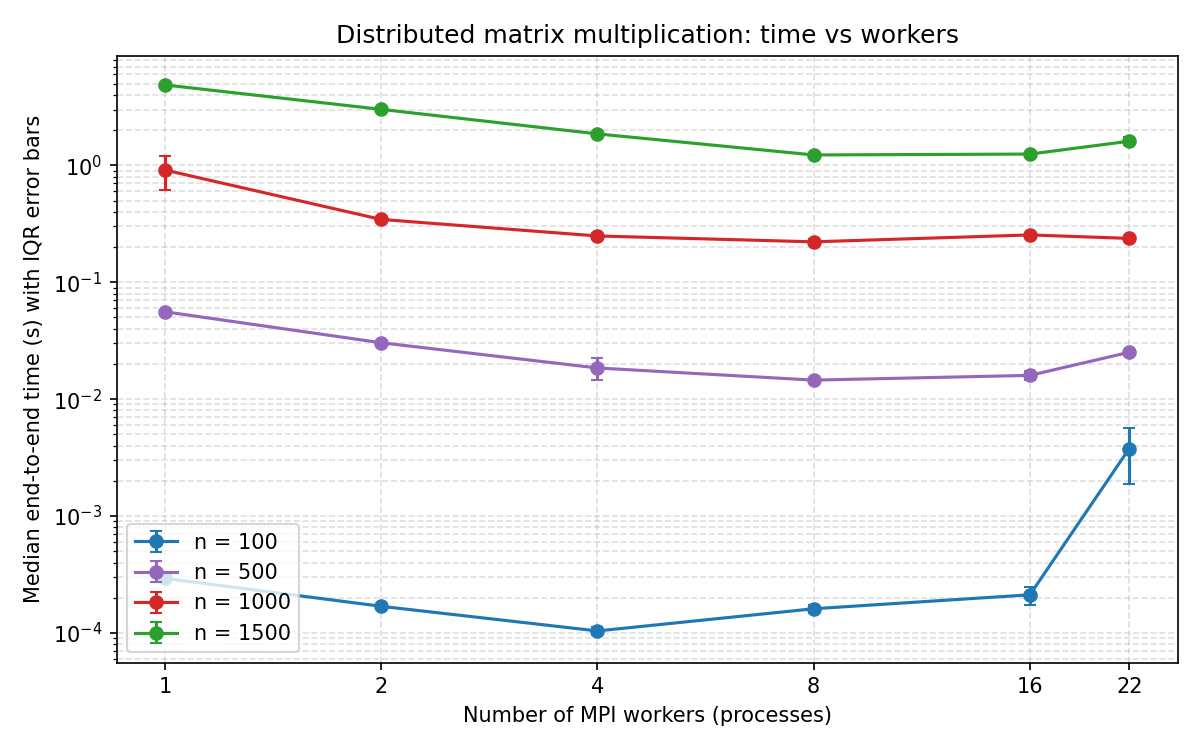
\includegraphics[width=0.9\textwidth]{plot_time_vs_workers_act4.png}
\caption{End-to-end time (s, log scale) vs.\ number of MPI workers for
$n \in \{100, 500, 1000, 1500\}$, with IQR error bars.}
\label{fig:time-workers}
\end{figure}

\textbf{Analysis:} As observed in Figure~\ref{fig:time-workers}, execution
time drops steeply as workers are added and then flattens: for $n = 1000$
the end-to-end time falls from 1092 ms (sequential) to 222 ms at $p = 8$ and
then stops improving (254 ms at $p = 16$, 237 ms at $p = 22$). For
$n = 1500$ the minimum is reached at $p = 8$ (1.227 s versus 7.081 s
sequential) and reverses at $p = 22$ (1.609 s) as communication grows. The
smallest problem ($n = 100$, bottom curve) is dominated by process
management: its time actually increases beyond $p = 4$, exactly as predicted
by H2. The IQR error bars are small except at MPI $p = 1$, where the
turbo-window effect described above is visible.

\subsubsection{Speedup Analysis}
\label{sec:speedupfig}

\begin{figure}[h]
\centering
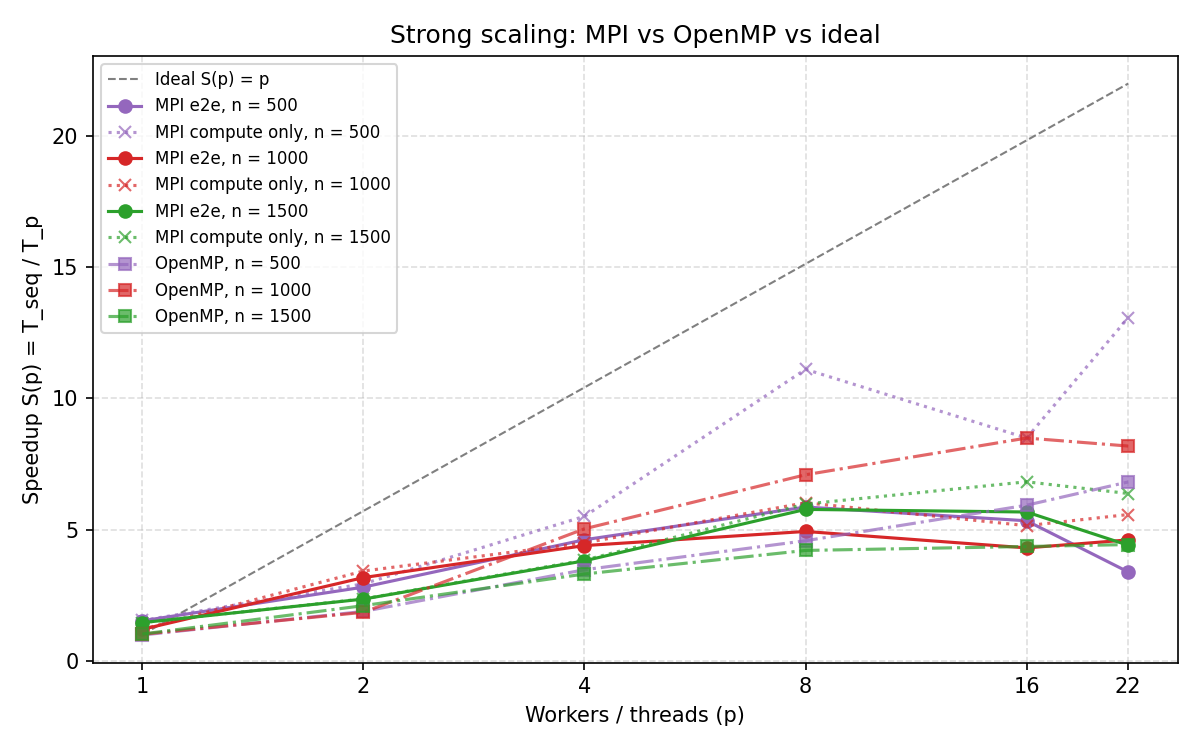
\includegraphics[width=0.9\textwidth]{plot_speedup_vs_workers_act4.png}
\caption{Speedup $S(p) = T_{\mathrm{seq}}/T_p$ (median end-to-end times)
vs.\ worker/thread count for $n \in \{500, 1000, 1500\}$, against the ideal
line $S(p) = p$. Solid lines: MPI end-to-end; dotted: MPI compute phase
only; dash-dotted: OpenMP reference.}
\label{fig:speedup}
\end{figure}

\textbf{Analysis:} Figure~\ref{fig:speedup} plots the speedups against the
ideal linear line. All curves bend away from the ideal early and peak at
$p = 8$: $S = 4.93$ ($n = 1000$) and $S = 5.77$ ($n = 1500$), after which
adding workers does not help (H1 confirmed). The compute-only curves keep
rising slightly longer (up to $6.82\times$ at $n = 1500$, $p = 16$) because
they exclude the growing transfer and gather phases; the gap between the
compute-only and end-to-end curves at $p = 16$--$22$ \emph{is} the
communication cost. The OpenMP reference (dash-dotted) rises higher than MPI
for $n = 1000$ (peak $8.49\times$ at 16 threads) but is overtaken by MPI for
$n = 1500$ at $p = 4$--$16$, which is analyzed in
Section~\ref{sec:discussion}. Relative to the MPI single-process time the
pure distribution scaling peaks at $4.12\times$ ($n = 1000$) and
$3.97\times$ ($n = 1500$), both at $p = 8$.

\subsubsection{Parallel Efficiency Analysis}
\label{sec:efffig}

\begin{figure}[h]
\centering
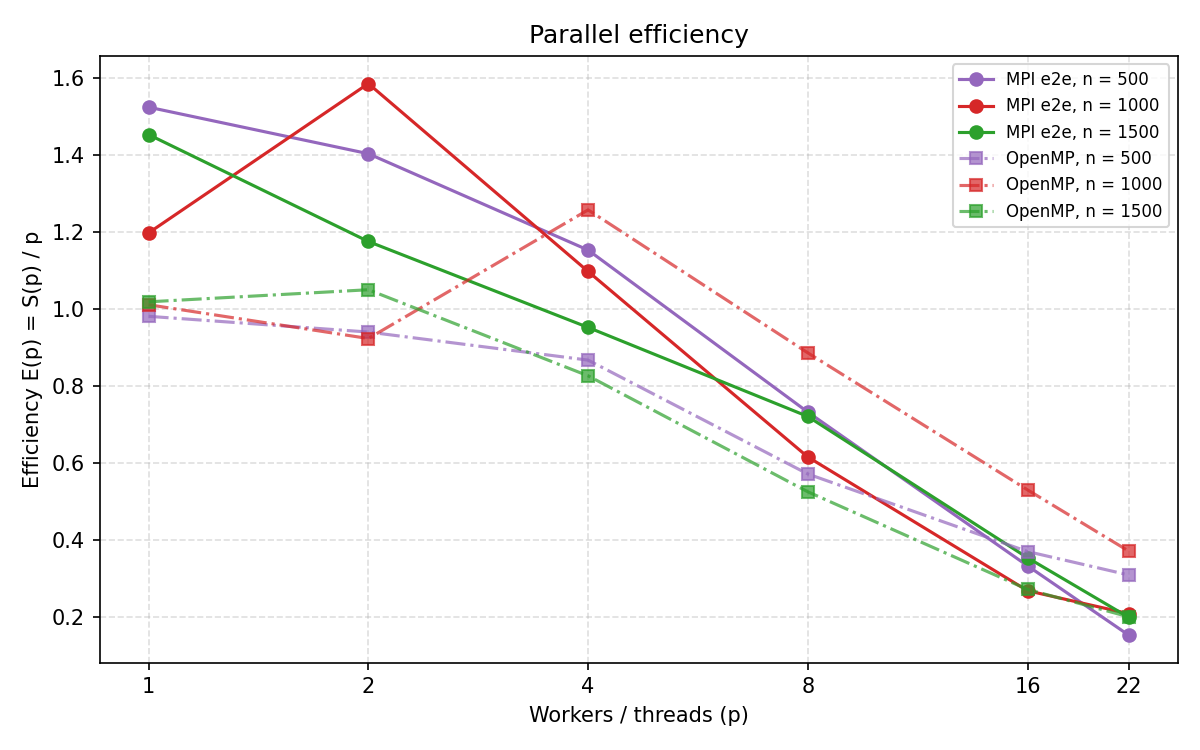
\includegraphics[width=0.9\textwidth]{plot_efficiency_act4.png}
\caption{Parallel execution efficiency $E(p) = S(p)/p$ relative to the
number of workers/threads (MPI end-to-end and OpenMP reference).}
\label{fig:efficiency}
\end{figure}

\textbf{Analysis:} As presented in Figure~\ref{fig:efficiency}, efficiency
stays at or above 1 up to $p = 2$--$4$ (with the superlinearity caveat of
Section~\ref{sec:data}), then decays as the speedup saturates: at the
best point ($p = 8$) about 62--72\% of the theoretical capacity is used
($n = 1000$ and $n = 1500$ respectively), and at $p = 22$ only about 20\%
remains. The OpenMP reference decays more slowly at high counts for
$n = 1000$ ($E = 0.53$ at 16 threads versus MPI's $E = 0.27$), consistent
with H3: shared memory avoids the per-process copies and collective
round-trips.

\subsubsection{Phase Breakdown}
\label{sec:phasefig}

\begin{figure}[h]
\centering
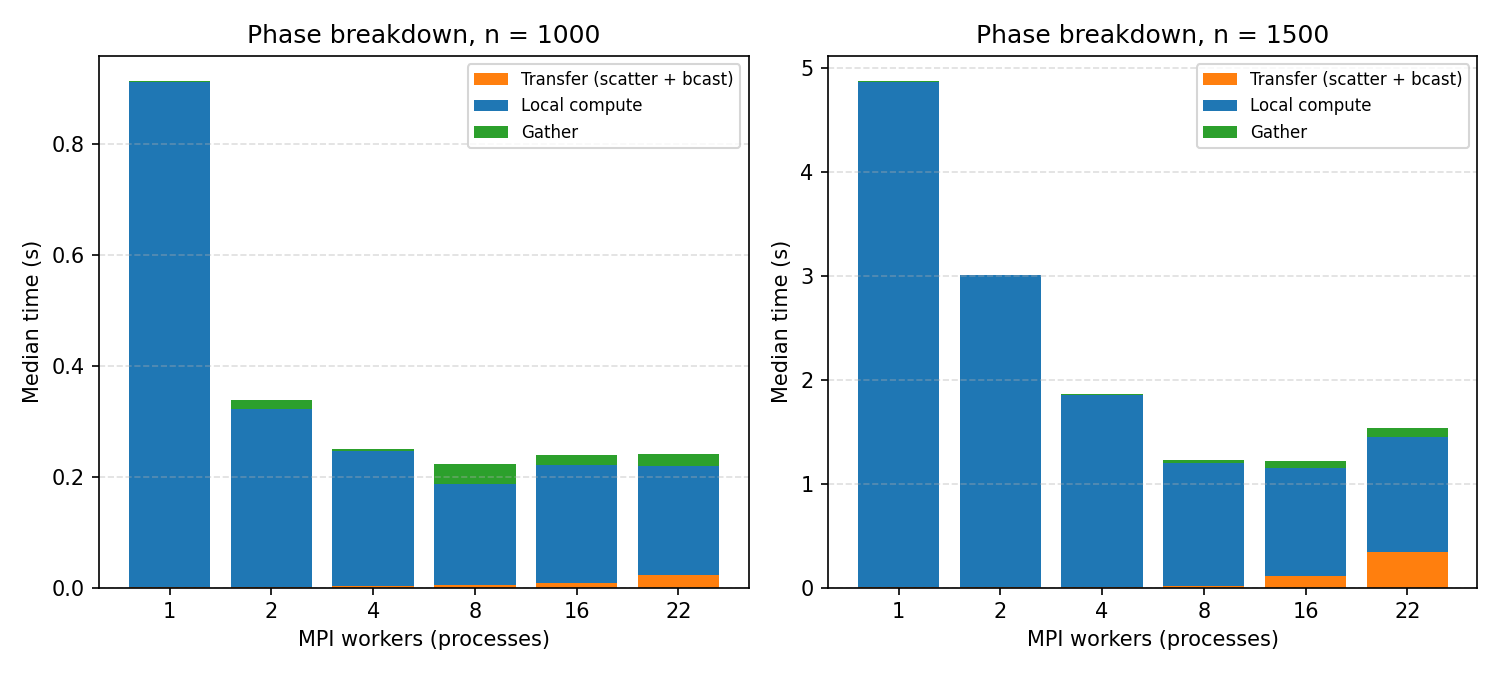
\includegraphics[width=0.95\textwidth]{plot_phase_breakdown_act4.png}
\caption{Stacked median phase times (transfer, local compute, gather) per
MPI worker count for $n = 1000$ and $n = 1500$.}
\label{fig:phase}
\end{figure}

\textbf{Analysis:} Figure~\ref{fig:phase} decomposes the end-to-end time.
At low worker counts the bars are almost entirely compute (99\%+,
Table~\ref{tab:phases}), so the distributed version behaves like a
shared-memory one. From $p = 16$ the transfer component (Scatterv of A plus
Bcast of B) becomes visible (8.8\% at $n = 1500$) and at $p = 22$ it
reaches 21.1\% (0.339 s), while the gather adds another 5.1\%. The compute
phase itself stops shrinking after $p = 8$ (1.186 s at $p = 8$ versus
1.111 s at $p = 22$), because the transfer is never overlapped with
computation in the current implementation and each worker also loses memory
bandwidth as more workers share the memory system. This confirms H1 and H2:
the saturation is communication- and
bandwidth-limited, not computation-limited.

\subsubsection{Method Comparison}
\label{sec:methodfig}

\begin{figure}[h]
\centering
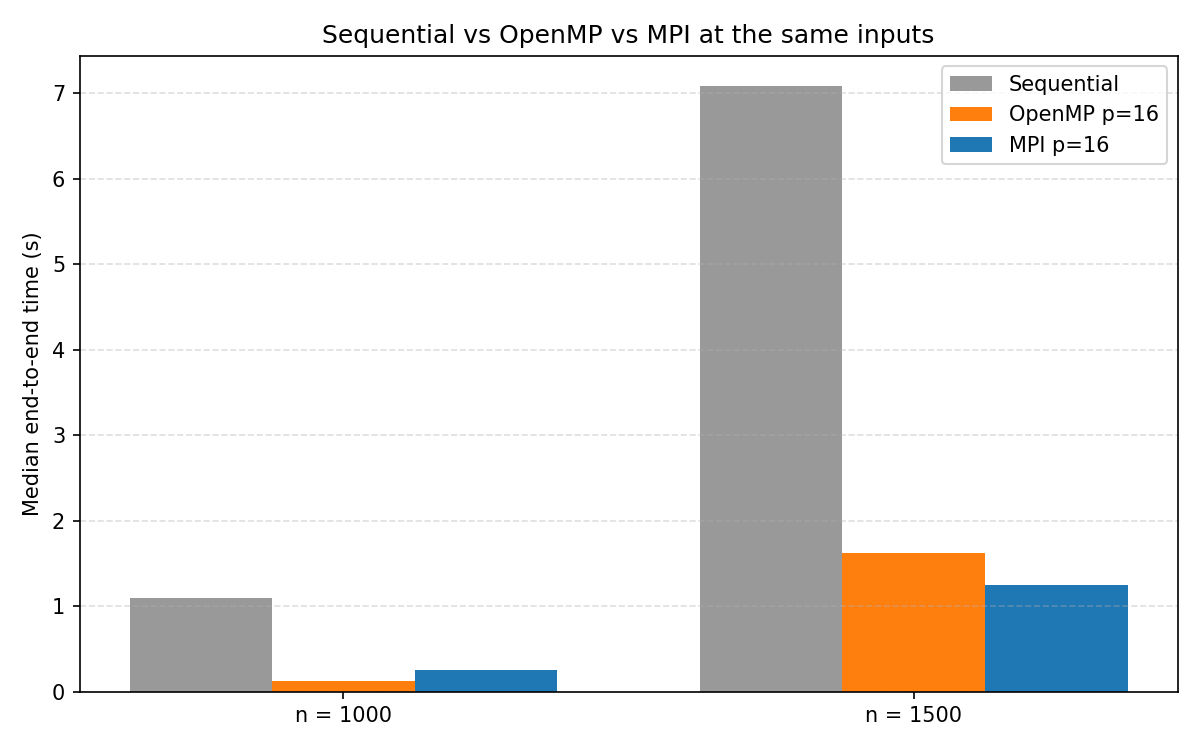
\includegraphics[width=0.9\textwidth]{plot_method_comparison_act4.png}
\caption{Median end-to-end time of sequential, OpenMP ($p=16$) and MPI
($p=16$) at the same inputs ($n = 1000$ and $n = 1500$).}
\label{fig:methods}
\end{figure}

\textbf{Analysis:} Figure~\ref{fig:methods} compares the three methods at a
fixed worker count. At $p = 16$ and $n = 1000$ the OpenMP version is about
twice as fast as MPI (129 ms versus 254 ms), while at $n = 1500$ MPI is
faster (1.249 s versus 1.626 s). The same crossover appears when comparing
each method at its own best point: OpenMP peaks at $8.49\times$
($n = 1000$), MPI at $5.77\times$ ($n = 1500$), where MPI is $1.30\times$
faster than the best OpenMP configuration (1.227 s versus 1.599 s).

\section{Analysis and discussion}
\label{sec:discussion}

\subsection{Observed performance comparison}
\label{sec:perfcompare}

The experimental results align closely with the architectural
characteristics of the execution environment:
\begin{itemize}
\item \textbf{Strong scaling saturation:} Both MPI and OpenMP saturate at
$p = 8$--$16$ (H1). The maximum MPI end-to-end speedup is $4.93\times$
($n = 1000$) and $5.77\times$ ($n = 1500$), giving efficiencies of
$\eta = 5.77 / 8 \approx 72\%$ at the sweet spot and $\eta \approx 20\%$ at
$p = 22$. Fitting the observed speedups at $p = 8$ yields an effective
serial-plus-overhead fraction of 6--9\%, similar to the OpenMP reference
fitted the same way (6--8\%); fitted at $p = 22$ it grows to 18--19\%,
because Amdahl's law absorbs the growing communication term as ``serial''.
Compared with Activity~3, where OpenMP saturated at 5--9\%, the MPI
saturation is therefore dominated by collectives and per-process overhead
rather than by thread scheduling.
\item \textbf{Data-layout effect (why $S(1) > 1$):} The MPI kernel runs
$1.20$--$1.52\times$ faster than the sequential baseline even with a single
process (Table~\ref{tab:cross}, $p = 1$ column): it multiplies packed
contiguous buffers, while the baseline walks rows allocated individually
(row-pointer storage with per-row indirection and heap placement). This is
why the report also quotes $S_{\mathrm{MPI1}}(p)$ (peaks $4.12\times$ /
$3.97\times$): part of the apparent ``parallel'' speedup at low $p$ is
layout, not distribution. The two effects are separated in every table.
\item \textbf{Communication cost:} The broadcast of the full B matrix is
the dominant transfer term: logically $n^2 \cdot 8 \cdot (p-1)$ bytes
($\approx$378 MB at $n = 1500$, $p = 22$). Because every worker needs every
column of B to compute its rows of C under 1-D row partitioning, this cost is
structural to the chosen partitioning, not an implementation accident. It is
also why the $n = 1500$ e2e time reverses after $p = 8$
(Table~\ref{tab:phases}): communication grows while compute no longer
shrinks. The current implementation performs no overlap --- transfer,
compute and gather run strictly in sequence --- so every extra byte of
broadcast is added verbatim to the end-to-end time.
\item \textbf{MPI vs.\ OpenMP (H3):} On one machine, OpenMP wins at
$n = 1000$ (up to $8.49\times$ versus $4.93\times$): threads share one copy
of B in the last-level cache and pay no collectives. At $n = 1500$ the
ranking inverts for $p = 4$--$16$: the packed contiguous buffers give MPI a
$1.45\times$ single-process advantage over the row-pointer OpenMP kernel,
which outweighs the collective cost of the tested counts. Both effects are
consistent with H3 and with the measurements; they are properties of this
machine and these sizes, not a general ranking of the frameworks.
\item \textbf{Small-problem overhead:} At $n = 100$ the e2e time grows
after $p = 4$ and collapses to $S = 0.11$ at $p = 22$ (3.78 ms, of which
1.9 ms is transfer): process launch, collective latency and measurement
noise dominate a sub-millisecond computation (H2 confirmed).
\item \textbf{Memory per worker:} The reported working set is the maximum
over workers: 129 MB at $n = 1500$, $p = 1$, decreasing to 97 MB at
$p = 22$ (constant full-B copy plus $1/p$ row blocks plus runtime). The
sequential/OpenMP processes hold all three matrices ($\approx$80 MB). All
values are two orders of magnitude below the declared 4 GB budget, and no
configuration came close to the 5 minute time budget (largest 7.49 s).
\item \textbf{Synchronization:} The 1-D partitioning gives every worker
disjoint rows of C and its private copy of A's block and B, so no locks or
atomics are needed inside the kernel; correctness reduces to the collective
calls, and the elementwise difference against the sequential reference is
exactly zero for all 260 measurements.
\end{itemize}

\subsection{Measurement reliability and environment factors}
\label{sec:reliability}

The methodology incorporated 5 official repetitions preceded by explicit
warm-up phases to minimize cold-start anomalies and transient system noise.
Furthermore, utilizing the median alongside the interquartile range (IQR)
guarantees robustness against isolated outliers caused by background
operating system tasks. The variability is small for most configurations
(IQR $\leq 6.5\%$ of the median for $n = 1000$), except MPI $p = 1$
(32.7\%, turbo-window straddling) and OpenMP $p = 2$ (26.0\%, same effect);
the smallest sizes have measurement noise comparable to their runtime and
should not be used for scaling conclusions. Two environment factors were
identified and controlled or documented: (1) the Balanced power plan caps
sustained single-thread throughput after the initial boost window, so all
official runs used the High Performance plan and warm-ups; (2) background
applications (browser, launcher, chat) were running during the campaign and
contribute to the residual scatter visible in a few configurations. Microsoft
MPI applies its own affinity policy on Windows 11, but OpenMP thread
placement remains OS-dependent, and CPU frequency/turbo states were only
controlled through the power plan, not pinned. All transfers are intra-host
shared-memory messages, so no conclusion about real network performance can
be drawn; only logical byte counts are reported. The conclusions are
therefore limited to the configurations actually measured (single machine,
single compiler, $n \leq 1500$, 1-D row partitioning without cache blocking
or 2-D decomposition, local multi-worker execution authorized by the
professor).

\section{Benchmarking and profiling tools}
\label{sec:tools}

\begin{itemize}
\item \textbf{Used in the project:}
\begin{itemize}
\item \textit{Timing \& Metrics:} \texttt{QueryPerformanceCounter} for
high-resolution wall-clock timing of each phase, and the process API
\texttt{GetProcessMemoryInfo} (\texttt{psapi}) for per-process memory in C,
reduced with \texttt{MPI\_Gather}.
\item \textit{Compilation:} \texttt{mpicc} (MSYS2 \texttt{msmpi} package)
wrapping gcc 16.2.0 with \texttt{-O3 -fopenmp}; \texttt{mpiexec} from
Microsoft MPI 10.1.12498.52.
\item \textit{Data Processing \& Visualization:} Python scripts utilizing
\texttt{pandas} for data unification and \texttt{matplotlib} for automated
plot generation and IQR variability computation; \texttt{numpy} as
correctness reference.
\end{itemize}
\item \textbf{Recommended for advanced analysis:}
\begin{itemize}
\item \textit{For MPI:} the Intel MPI Benchmarks (\texttt{IMB}) to
characterize the intra-host (and, on a real cluster, network) transport;
\texttt{mpiP} or Score-P/Scalasca for collective-level communication
profiles; TAU for phase timelines.
\item \textit{For C/OpenMP:} Linux \texttt{perf} (cycles, cache misses,
bandwidth counters) or Intel VTune Profiler for thread scaling and memory
access analysis on the reference machine.
\item \textit{For correctness under optimization:} extended self-tests with
random sizes and non-divisible worker counts (the campaign already
exercises non-divisible cases such as $p = 16$ for $n = 1000$).
\end{itemize}
\end{itemize}

\section{Optimization recommendations}
\label{sec:opt}

To overcome the performance bottlenecks identified during benchmarking,
several optimization strategies can be implemented:
\begin{itemize}
\item \textbf{Partitioning:} Move to a 2-D block partitioning of C so each
worker receives only its $\sqrt{p} \times \sqrt{p}$ block of B instead of
the full matrix: at $n = 1500$, $p = 22$ each worker would hold
$\approx$3.8 MB of B rather than 18 MB, shrinking the broadcast term from
$n^2 \cdot 8 \cdot (p-1)$ logical bytes to roughly
$n^2 \cdot 8 \cdot (p-1)/\sqrt{p}$, at the cost of two rounds of
\texttt{MPI\_Alltoall}.
\item \textbf{Overlap:} Replace the blocking collectives with
\texttt{MPI\_Ibcast}/\texttt{MPI\_Isend}/\texttt{MPI\_Irecv} and compute the
rows of C whose B rows have already arrived (pipeline), hiding a large part
of the 21\% transfer share observed at $p = 22$.
\item \textbf{Local kernel:} Combine the distributed version with the
vectorized i-k-j kernel validated in Activity~3; the local compute phase is
still the dominant term at $p \leq 16$, and the two optimizations act on
different resources.
\item \textbf{Data layout:} Eliminate the row-pointer indirection of the
sequential/OpenMP baseline (pack once into contiguous buffers outside the
timed region) so that the three methods share the same layout and the
speedup measures distribution alone.
\item \textbf{Transport:} Use persistent collectives or derived datatypes
for the Scatterv/Gatherv of rows; MS-MPI already applies CPU-set affinity
on Windows 11, so verify worker placement rather than re-pinning it.
\item \textbf{Scaling further:} Repeat the campaign on a real multi-host
cluster (the current data cannot say anything about network latency), and
evaluate larger matrices beyond the shared L3 together with the 2-D
partitioning.
\end{itemize}

\section{Conclusions}
\label{sec:concl}

\begin{itemize}
\item \textbf{Performance findings:} Within the evaluated scope
($n \in \{100, 500, 1000, 1500\}$, $p \in \{1, \dots, 22\}$), the MPI
distribution delivers up to $5.77\times$ end-to-end speedup ($n = 1500$),
saturating at $p = 8$ with efficiency $0.62$--$0.72$ and falling to
$\approx 0.20$ at $p = 22$; the practical sweet spot is $p = 8$. The
compute-only phase reaches $6.82\times$ ($n = 1500$, $p = 16$), so the gap
to the end-to-end curve is pure communication.
\item \textbf{Communication finding:} Transfer grows from negligible
($<1\%$ at $p \leq 8$) to 21.1\% of the end-to-end time at $p = 22$
($n = 1500$), dominated by broadcasting the full B matrix --- a structural
cost of 1-D row partitioning, quantified as
$n^2 \cdot 8 \cdot (p-1)$ logical bytes ($\approx$378 MB at $n = 1500$,
$p = 22$). This is the main reason scaling reverses beyond $p = 8$.
\item \textbf{Comparison finding:} On this single machine, OpenMP remains
the best choice at $n = 1000$ ($8.49\times$ versus $4.93\times$), while MPI
with packed buffers wins for $n = 1500$ (up to $1.30\times$ faster than the
best OpenMP configuration); the packed-versus-row-pointer layout effect
($1.20$--$1.52\times$ at $p = 1$) is isolated and reported separately so it
is not mistaken for distribution speedup.
\item \textbf{Experimental rigor:} Ensuring reproducible benchmarks
required identical input matrices across methods, warm-up phases, multiple
official repetitions with median/IQR statistics, a documented power-plan
control, checksum validation against both the sequential reference and
NumPy, and an explicit separation of workers (MPI processes) from threads
(OpenMP) with the local multi-worker configuration labeled and authorized.
\item \textbf{Open limitations:} How the 1-D partitioning compares with a
2-D decomposition, how the curves shift on a real network, how much of the
communication can be hidden by non-blocking collectives, and whether the
layout advantage persists on a homogeneous server CPU remain unresolved.
\item \textbf{AI Collaboration Disclosure:} In accordance with transparent
academic practices, OpenCode (a large-language-model-based CLI assistant)
was utilized during the development of this project. Its purpose was
strictly limited to assisting with technical writing, structuring the
academic report in LaTeX, debugging compilation errors, and refining the
data analysis methodology. All benchmarking executions, code
implementations, and final validations were independently performed and
verified by the author, who also generated all figures locally and checked
every reported number against the raw CSV measurements.
\end{itemize}

\end{document}
